\chapter{实现}

\section{Schedule}

不能支持嵌套task,用pre yield变量来控制。

\section{内存}

提供什么接口

使用场景
\begin{easylist}[itemize]
    & core private memory
    & sche\_task
    & RDMA
    & buffer\_t
    && libnvme
    & little object
    & ring
\end{easylist}

采用buddy算法管理连续内存分配

动态化

用面向对象的方式处理,每个core对应一个MR对象。public的也是如此。

每个对象内嵌一个buddy对象管理hugepage的分配、释放。
另外,从core的MR里,利用buddy算法分配连续内存,用于ring等小对象。

禁止在一个core内malloc,由另外一个core进行free。

\subsection{buffer}

\begin{center}
    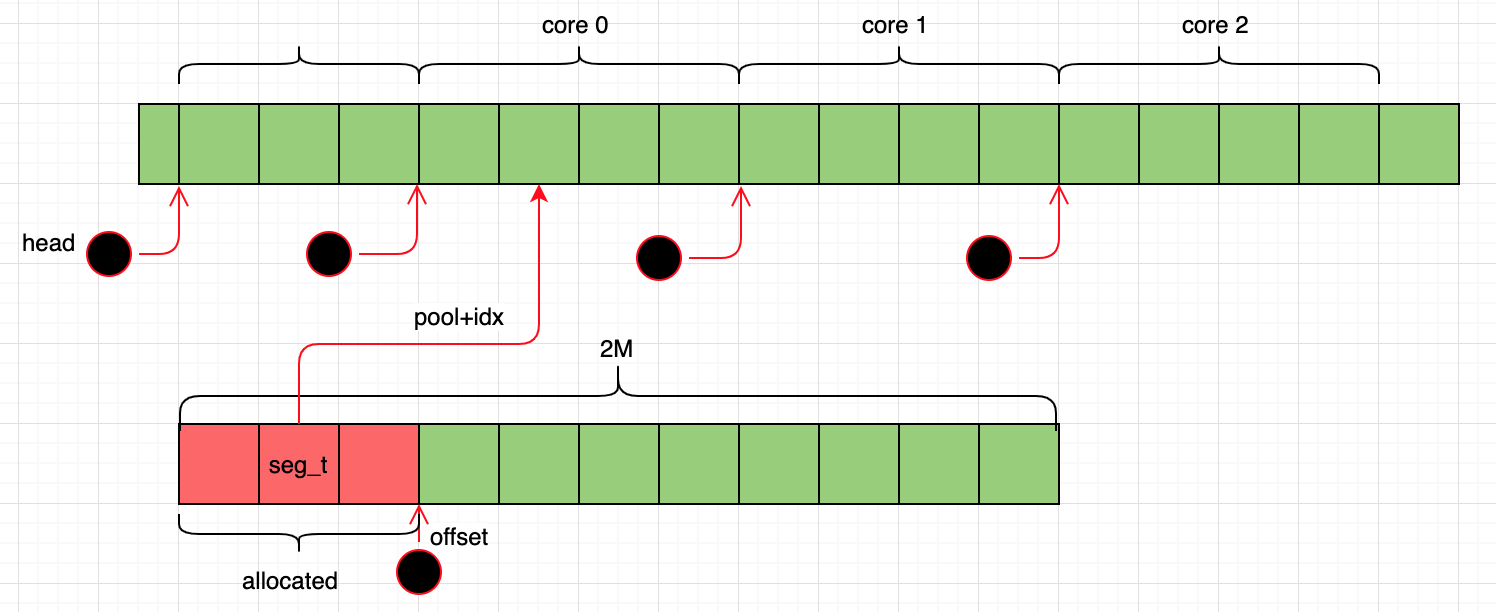
\includegraphics[width=10cm]{../imgs/buffer-t.png}
\end{center}

buffer的每个seg都包含有虚拟地址和物理地址。

\subsection{NVMe}

NVMe为什么需要物理地址?

\subsection{RDMA}

每个连接$1024*512$内存。
